% Resumen para la reunion del 12-10-2026. Compilar con pdfLaTeX. Usa las tres imagenes de esta carpeta.
\documentclass[11pt,a4paper]{article}
\usepackage[utf8]{inputenc}
\usepackage[T1]{fontenc}
\usepackage[spanish,es-tabla,es-nodecimaldot]{babel}
\usepackage[a4paper,margin=2.2cm]{geometry}
\usepackage{graphicx}
\usepackage{float}
\usepackage{booktabs}
\usepackage{enumitem}
\setlist{itemsep=1pt,topsep=3pt}
\pagestyle{plain}

\begin{document}

\begin{center}
  {\Large\bfseries Generador peine con SDR: estado al 12 de octubre de 2026}\\[4pt]
  Martín Ledesma -- Compatibilidad Electromagnética (FIUBA)\\
  Resumen para la reunión previa a la medición en el CETEM (martes 13 de octubre)
\end{center}

\section*{1. Qué hay construido}

Un generador peine hecho con una bladeRF 2.0 micro xA9 y GNU Radio, para verificar la cadena de emisiones radiadas del CETEM y seguir su continuidad en el tiempo.

\begin{itemize}
  \item 24 líneas de 60 a 980~MHz, una cada 40~MHz. La SDR emite una línea por vez; el receptor las acumula con MAX HOLD.
  \item Un solo tono por portadora, con la portadora 10~MHz por encima de la línea, a 40~MSPS.
  \item Cada línea está 6~s encendida y 6~s apagada; el salto de frecuencia se hace durante el silencio. Una pasada completa dura 4~min~48~s.
  \item Calibración por cable contra un analizador: el programa lee la captura (.csv), busca el pico de cada línea y la lleva a 0~dBm. Se guarda en un archivo y se importa con un botón. Admite retoque manual por línea.
  \item Opción de subir todas las líneas 3~dB (da +2,3~dBm de media: la placa empieza a comprimir).
\end{itemize}

\section*{2. Resultado por cable}

\begin{figure}[H]
  \centering
  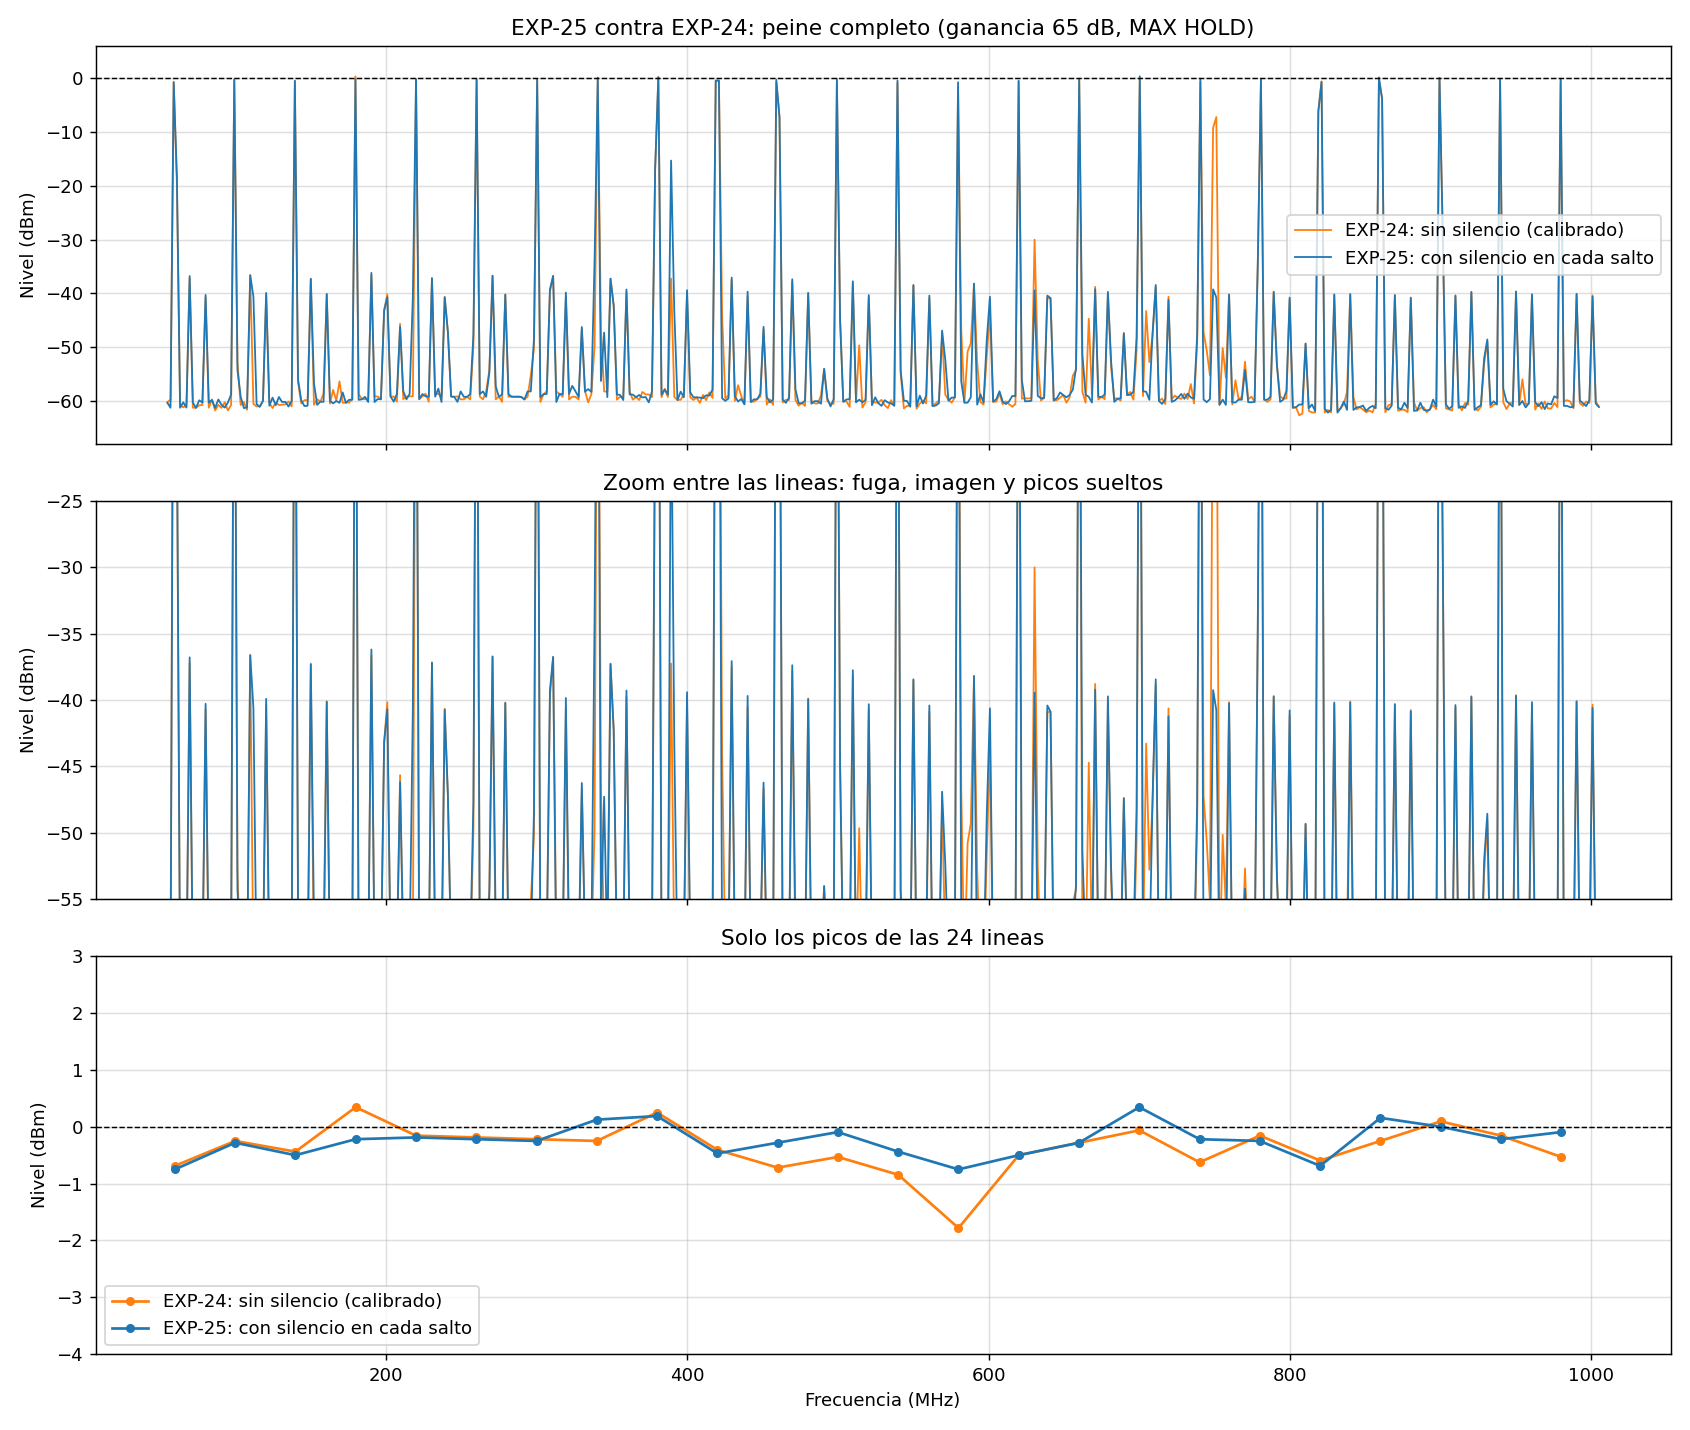
\includegraphics[width=0.92\textwidth]{fig_conducido_exp25.png}
  \caption{Peine calibrado medido por cable con la tinySA (MAX HOLD). Naranja: sin silencio en los saltos. Azul: con silencio.}
\end{figure}

\begin{itemize}
  \item Las 24 líneas quedan entre $-0{,}8$ y $+0{,}3$~dBm: planitud de 1,1~dB, desvío de 0,28~dB.
  \item Entre las líneas queda solo lo débil: fuga de portadora ($-36$ a $-40$~dBm), imagen (40~dB bajo la línea) y el triple de la portadora ($-46$ a $-49$~dBm).
  \item Por qué 40~MHz: el mezclador de la SDR repite cada línea alrededor de los armónicos impares de la portadora, entre 9 y 28~dB por debajo. Con este espaciado y esta posición de la portadora, esas repeticiones caen justo sobre otras líneas del peine y MAX HOLD las tapa. Con líneas cada 50~MHz haría falta más ancho de banda del que el USB de la PC sostiene.
\end{itemize}

\section*{3. Resultado radiado (prueba en casa, 12 de octubre)}

SDR con antena telescópica de 30~cm totalmente extendida; tinySA a 2~m con una antena de 10~cm; líneas calibradas a 0~dBm; sin blindaje.

\begin{figure}[H]
  \centering
  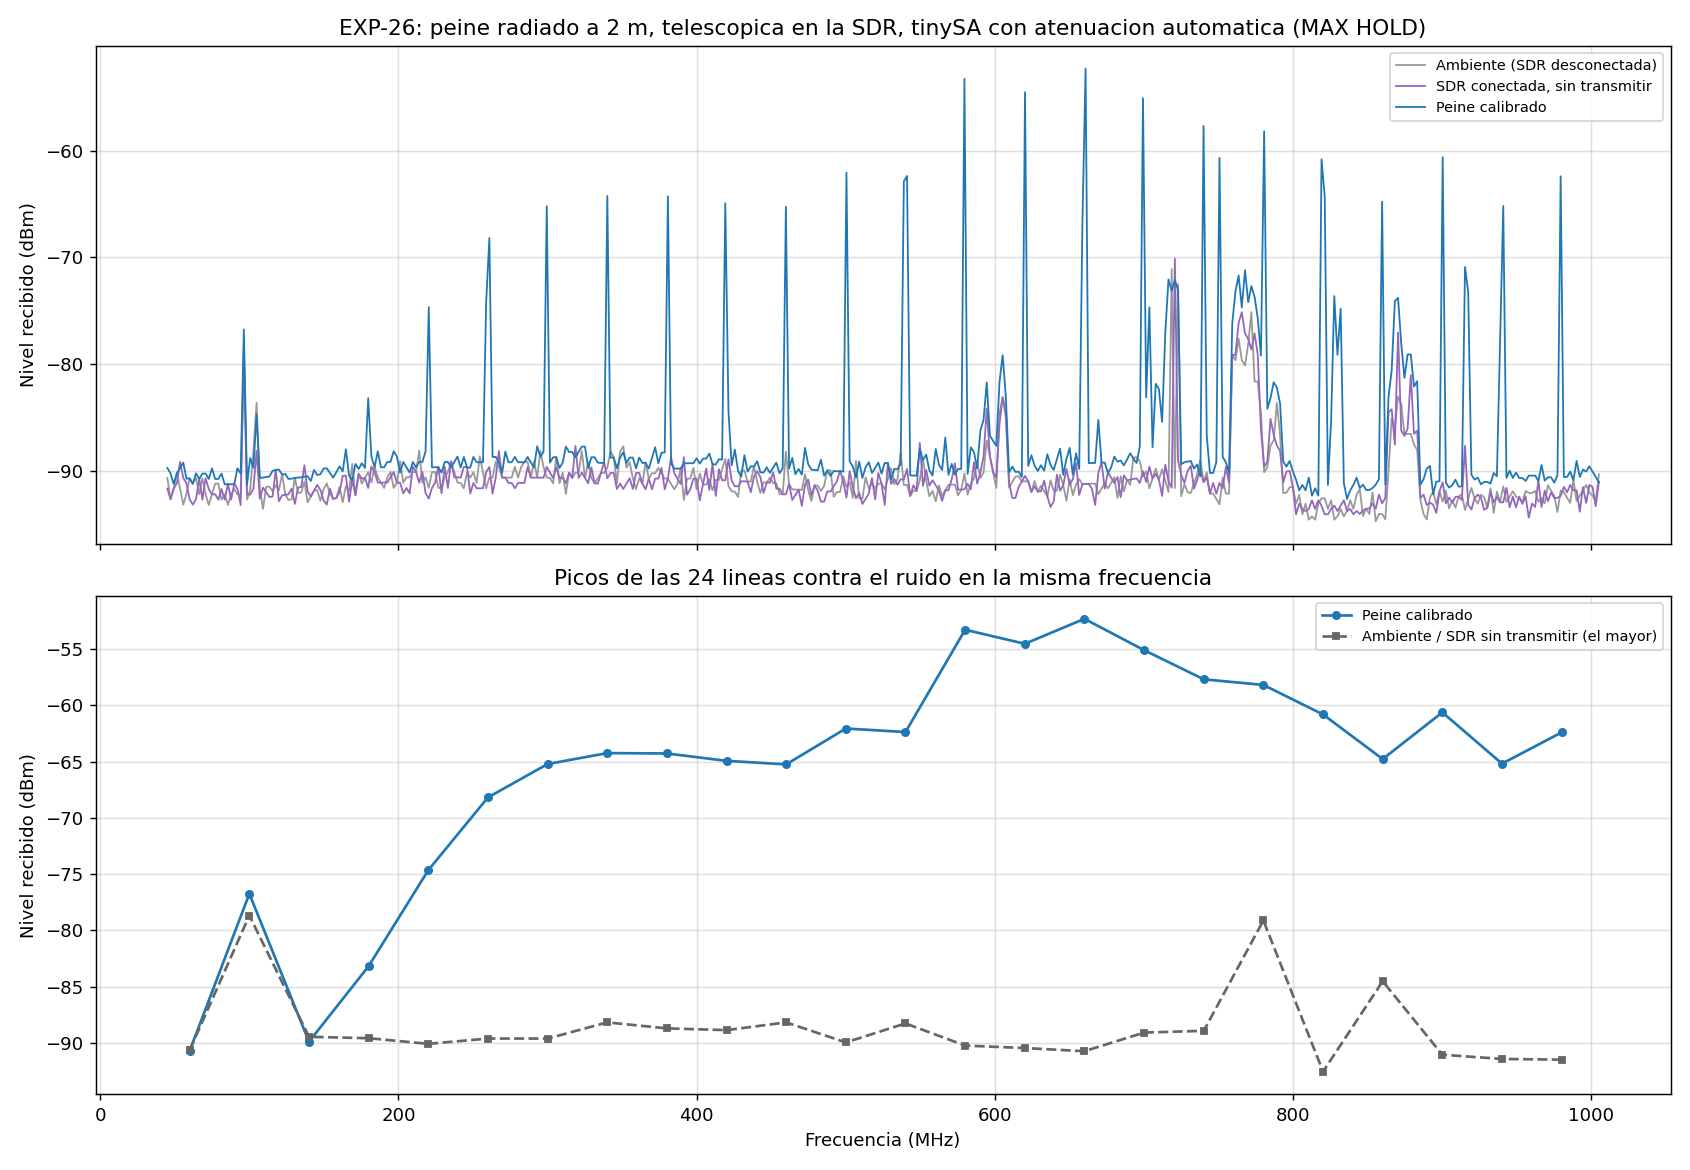
\includegraphics[width=0.92\textwidth]{fig_radiado_exp26.png}
  \caption{Peine radiado a 2~m. Arriba: trazas completas. Abajo: nivel de cada línea contra el ruido en esa frecuencia.}
\end{figure}

\begin{itemize}
  \item 20 de las 24 líneas se reciben 10~dB o más por encima del ruido, y 18 con 20~dB o más (hasta 38~dB).
  \item No sirvieron cuatro líneas bajas: 60 y 140~MHz no se ven, 100~MHz queda tapada por FM y 180~MHz tiene solo 6~dB. La antena de 30~cm irradia poco ahí.
  \item La SDR encendida sin transmitir no agrega nada claro sobre el ambiente, aun sin blindaje.
  \item En el ambiente de una casa aparecen FM y celular; en la cámara no deberían estar.
\end{itemize}

\section*{4. Lo que falta o no está resuelto}

\begin{itemize}
  \item \textbf{No se comprobó por aire que la calibración por cable se traslade}, ni la repetibilidad al desmontar y volver a montar: faltó tiempo para esas capturas. El procedimiento incluye el paso de repetibilidad en la primera visita.
  \item \textbf{Líneas por debajo de 220~MHz:} dudosas con esta antena. Se verá con el receptor del CETEM, que es más sensible.
  \item \textbf{Pico suelto en 750~MHz:} aparece cada tanto, a veces casi tan alto como una línea. Es la frecuencia de una portadora, no una línea del peine. Causa sin identificar; se sospecha de la recalibración automática del chip.
  \item \textbf{Cable USB de la cámara:} el programa necesita USB~3 (40~MSPS) y la placa se alimenta por ese cable. No se pudo probar con un cable largo. En una prueba la comunicación USB se cortó una vez, a los 15~minutos, con el cable original de medio metro.
  \item \textbf{Por encima de 1~GHz} salen armónicos de las líneas: la SDR no tiene filtro de salida.
  \item \textbf{Firmware:} sin actualizar, como se acordó.
\end{itemize}

\section*{5. Para la medición del martes}

\begin{itemize}
  \item Procedimiento RE-TP-001 escrito sobre el esquema de la cátedra (13 páginas), con geometría fija y la maximización como paso de única vez.
  \item Criterio de continuidad propuesto: hasta $\pm$3~dB conforme; entre 3 y 6~dB revisar y repetir; más de 6~dB no conforme. A confirmar con la repetibilidad medida ese día.
  \item Datos a completar en el laboratorio: modelo del receptor y de la antena, tiempo de barrido (tiene que ser menor a 3~s), y si el cable USB instalado es USB~3.
\end{itemize}

\end{document}
